\section{A Performance Model for \glsentryshort{3G} \glsentryshort{RRC} States}\label{sec:network:performance_model}
The algorithm introduced in \refsec{sec:network:network_traces} can be used to infer the signalling frequency, power drain and \gls{QoE} of existing or prototyped applications.
However, in order to study the general impact of traffic, methods to derive said metrics from analytical traffic distributions are of interest.

In \refsec{sec:network:performance_model:analytical_model} we introduce an model allowing us to 
analyse both theoretical and empirical traffic models.
Then, in \refsec{sec:network:performance_model:numerical_examples} we use this model to study the impact of traffic characteristic on metrics such as signalling intensity and power drain.

\subsection{Analytical Model}\label{sec:network:performance_model:analytical_model}
This section introduces a performance model for quantifying power drain against signalling load.
The model allows researchers and application developers to evaluate analytical and empirical traffic distributions, deriving metrics for signalling and power drain in order to predict the impact of yet unimplemented applications or planned network configurations.

After presenting the system description, we derive the state distribution and the average frequency of state transitions for a Two State Model, e.g. for proprietary fast dormancy implementations of smart-phone vendors~\cite{NSN2011}. 
Afterwards, we extend the model to include \gls{RRC_FACH} for regular \gls{3G} networks.
Finally, we define simple metrics for signalling load and power drain.

\newcommand{\PacketIAT}{A}

\subsubsection*{System Description}\label{sec:network:performance_model:analytical_model:system_description}
We consider a \gls{UE} which sends and receives a sequence of data packets via a \gls{3G} \gls{UMTS} network.
As discussed in \refsec{sec:network:background:umts_rrc}, the arrival process of the packet transmissions determines the \gls{RRC} states of the \gls{UE}.
However, the direction of packets, i.e. whether they originate from the \gls{UE} or the \gls{NodeB}, has no impact on the \gls{RRC} states, as the states depend solely on traffic activity.
Due to the high impact of \gls{RRC} states on traffic patterns, we do not consider packet sizes in this model.
In real \gls{UMTS} networks very small packets might be treated differently for \gls{RRC} states, but we neglect this both for simplicity reasons and as the impact of packet sizes is highly network operator specific~\cite{Qian2010a}.
Furthermore, \gls{RRC} state transitions are complex procedures depending on implementation details of the \gls{UE}, the specific \gls{UMTS} release, and the configurations by the network operator.
In order to keep our model simple, but realistic, we reduce the set of standardized \gls{RRC} states and the state transition triggers in the following ways. 

In a first step we consider the Two State Model: \gls{RRC_idle} and \gls{RRC_DCH} as shown in \reffig{fig:network:background:rrc_state_machines:two_states}.
The \gls{UE} switches to \gls{RRC_DCH} to transmit or receive data and after an inactivity period of duration \gls{TDCH}, it switches back to \gls{RRC_idle}. 
The motivation for the two states \gls{RRC} scenario is twofold.
First, it serves for illustration purposes.
We derive the model step-by-step in this simple scenario to explain the ideas behind the equations.
Then, the ideas can be easily transferred to the more complex Three State Model.
Second, the scenario is of practical relevance since proprietary implementations of the fast dormancy concept can be modeled as the Two State Model, as discussed in \refsec{sec:network:background:umts_rrc}.
Furthermore, this model is very similar to the one found in \gls{LTE} systems.
In \gls{LTE}, only a distinction between connected and disconnected states can be found, which maps to the \gls{RRC_idle} and \gls{RRC_DCH} states discussed in this model.

In our model we aggregate both packets sent and received by the \gls{UE} in the packet arrival process, which is assumed to be a renewal process, i.e. a process  with identical and independently distributed inter-arrival times, described by the random variable \(\PacketIAT\) as shown in~\reffig{fig:network:performance_model:system_description:arrival_process}.
Thus, the probability that the time between two consecutive packets is at most \(t\) is \(P(\PacketIAT \leq t) = \PacketIAT(t)\).
This assumption is validated in \refsec{sec:network:performance_model:validations} using the application measurements obtained in \refsec{sec:network:network_traces:numerical_results}.

The packet arrivals determine the \gls{RRC} state of the \gls{UE} and the corresponding transitions. Therefore, the packet arrival process can be seen as a modulating process, c.f. \cite{TranGia1983,TranGia1988}, while the state and the signalling process represent modulated, i.e., resulting processes.

\begin{figure}
  \centering
  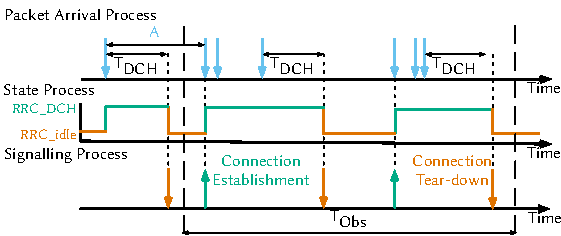
\includegraphics{network/performance_model/analytical_model/figures/arrival_process}
  \caption{Relation of packet arival process \(\PacketIAT\), state process, and signalling process in the Two State Model.}
  \label{fig:network:performance_model:system_description:arrival_process}
\end{figure}

\subsubsection*{Two State Model}\label{sec:network:performance_model:analytical_model:two_states}

\newcommand{\RRCState}{S}
\newcommand{\PacketIATDensity}{a}
\newcommand{\RRCStateRealization}{s}
\newcommand{\ObservationInterval}{T_{\text{Obs}}}
\newcommand{\ObservationPoint}{t^*}
\newcommand{\ObservationIntervalDensity}{q}
\newcommand{\ObservationIntervalLength}{\tau}
\newcommand{\NormalisationConstant}{c_0}
\newcommand{\NObservedPackets}{n_{\text{P}}}

\paragraph*{State Distribution}
First, we are interested in the state distribution \(P(\RRCState=\RRCStateRealization)\), i.e., the fraction of time the \gls{UE} spends in state \(\RRCStateRealization\in\{\gls{RRC_idle},\gls{RRC_DCH}\}\) for a given inter-packet time \(\PacketIAT\).
For this purpose, we define an observation interval \(\ObservationInterval\), depicted in \reffig{fig:network:performance_model:system_description:arrival_process}, which is assumed to be larger in orders of magnitude than the average packet inter-arrival time \(E[\PacketIAT]\).
In addition, we take the position of an outside observer who observes the state \(\RRCState\) at a random point in time \(\ObservationPoint\), uniformly distributed within the observation interval. 
Then the state distribution \(P(\RRCState=\RRCStateRealization)\) is the probability that the observer encounters the \gls{UE} in state \(\RRCState\) at the time \(\ObservationPoint\). 

We calculate this distribution as 
\begin{equation}
P(\RRCState=\RRCStateRealization)= 
  \int_{0}^\infty \ObservationIntervalDensity(\tau) \cdot 
  P(\RRCState=\RRCStateRealization \vert \PacketIAT = \ObservationIntervalLength) d\ObservationIntervalLength,
  \label{eq:network:performance_model:system_description:state_distribution} 
\end{equation} 
where \(\ObservationIntervalDensity(\ObservationIntervalLength)\) is the probability density that \(\ObservationPoint\) falls into an interval of length \(\ObservationIntervalLength\) and 
\(P(\RRCState=\RRCStateRealization) \vert \PacketIAT = \ObservationIntervalLength)\)
is the probability that the \gls{UE} is in state \(\RRCState\) under the condition that \(\ObservationPoint\) is within an interval of length \(\ObservationIntervalLength\).

First, we derive \(\ObservationIntervalDensity(\ObservationIntervalLength)\). 
This probability density has to be proportional to \(\PacketIATDensity(\ObservationIntervalLength)\) and to \(\ObservationIntervalLength\), where \(\PacketIATDensity(\ObservationIntervalLength)\) is the probability density function of the random variable \(\PacketIAT\). 
Therefore, we have that 
\(\ObservationIntervalDensity(\ObservationIntervalLength)=\PacketIATDensity(\ObservationIntervalLength)\cdot\ObservationIntervalLength\cdot \NormalisationConstant\)
with the proportionality constant \(\NormalisationConstant\).
Due to 
\(\int_0^\infty \ObservationIntervalDensity(\ObservationIntervalLength)d\ObservationIntervalLength=1\),
we have 
\(\NormalisationConstant=1/E[\PacketIAT]\)
, which leads to
\begin{equation*}
\ObservationIntervalDensity(\ObservationIntervalLength)=\frac{a(\ObservationIntervalLength) \cdot \ObservationIntervalLength}{E[\PacketIAT]}.
\label{eq:network:performance_model:system_description:state_distribution:observation_density}
\end{equation*}

Next, we derive the conditional probability
\(P(\RRCState=\RRCStateRealization \vert \PacketIAT = \ObservationIntervalLength)\)
that \(\ObservationPoint\) falls within a period with state \(\RRCState\) under the condition that the inter-packet time is
\(\PacketIAT = \ObservationIntervalLength\). 
We use the fact that \(\ObservationPoint\) is uniformly distributed within \(\ObservationIntervalLength\) and calculate the probability 
\(P(\RRCState = \gls{RRC_idle})\)
by considering the relevant cases:
\begin{equation}
P(\RRCState=\gls{RRC_idle}\vert \PacketIAT = \ObservationIntervalLength)=
\begin{cases} 
	0,  & \mbox{if } \ObservationInterval \leq \gls{TDCH} \\ 
    \frac{\ObservationIntervalLength - \gls{TDCH}}{\ObservationIntervalLength}, & \mbox{otherwise.}	 
\end{cases}
\end{equation}

Similarly, we obtain \(P(\RRCState = \gls{RRC_DCH})\) as:
\begin{equation}
P(\RRCState=\gls{RRC_DCH} \vert \PacketIAT = \ObservationIntervalLength)=
\begin{cases} 
	1,  & \mbox{if } \ObservationIntervalLength \leq \gls{TDCH} \\ 
    \frac{\gls{TDCH}}{\ObservationIntervalLength}, & \mbox{otherwise.}	 
\end{cases}
\label{eq:network:performance_model:system_description:state_distribution:conditional_probability_dch}
\end{equation} 

\paragraph*{Average Frequency of State Transitions}

\newcommand{\NStateTransitionsIdleToDCH}{n_{\gls{RRC_idle}\rightarrow\gls{RRC_DCH}}}
\newcommand{\NStateTransitionsDCHToIdle}{n_{\gls{RRC_DCH}\rightarrow\gls{RRC_idle}}}
\newcommand{\fStateTransitionsIdleToDCH}{f_{\gls{RRC_idle}\rightarrow\gls{RRC_DCH}}}
\newcommand{\fStateTransitionsDCHToIdle}{f_{\gls{RRC_DCH}\rightarrow\gls{RRC_idle}}}

Next, we estimate the average frequency of state transitions resulting from a given packet arrival process.
For that purpose, we consider again the observation interval \(\ObservationInterval\) and focus on the state transitions from \gls{RRC_idle} to \gls{RRC_DCH} since every switch from \gls{RRC_DCH} to \gls{RRC_idle} results in a switch vice-versa.
The expected number of observed packets during \(\ObservationInterval\) is 
\(E[\NObservedPackets]=\ObservationInterval/E[\PacketIAT]\). 
Furthermore, the probability that time between two consecutive packets exceeds the timer \(\gls{TDCH}\) is
\begin{equation} 
P(\PacketIAT > \gls{TDCH}) = 1 - P(\PacketIAT \leq \gls{TDCH}) = 1 - \PacketIAT(\gls{TDCH}).
\end{equation} 
The number of state transitions \(\NStateTransitionsIdleToDCH\) during \(\ObservationInterval\) directly corresponds to the number of inter-packet times exceeding \(\gls{TDCH}\) since an active connection is torn down after an inactivity period of \(\gls{TDCH}\).
Thus, the expected number is 
\begin{align*}
\begin{split}
E[\NStateTransitionsIdleToDCH] & = E[\NObservedPackets] \cdot P(\PacketIAT > \gls{TDCH})\\
	& = \frac{\ObservationInterval}{E[\PacketIAT]}\cdot (1-\PacketIAT(\gls{TDCH})). 
\end{split}
\end{align*} 
Hence, the expected frequency of state transitions is 
\begin{equation*}
E[\NStateTransitionsIdleToDCH]=\frac{1-\PacketIAT(\gls{TDCH})}{E[\PacketIAT]}.
\end{equation*}
The same holds also for the state transitions from \gls{RRC_DCH} to \gls{RRC_idle} and hence 
\(E[\fStateTransitionsDCHToIdle]=E[\fStateTransitionsDCHToIdle]\)
holds.

\subsubsection*{Three State Model}\label{sec:network:performance_model:analytical_model:three_states}
In this section we consider three states: \gls{RRC_idle}, \gls{RRC_DCH}, and \gls{RRC_FACH}.
Again, we assume that the \gls{UE} switches from \gls{RRC_idle} to \gls{RRC_DCH} whenever it transmits or receives data.
After an inactivity of \(\gls{TDCH}\) the \gls{UE} switches to \gls{RRC_FACH}, and after an additional inactivity of \(\gls{TFACH}\), it switches to \gls{RRC_idle}, as depicted in \reffig{fig:network:background:rrc_state_machines:three_states}.
This scenario usually occurs when the network controls the \gls{RRC} state of the \gls{UE} without proprietary connection tear-down mechanisms implemented on the \gls{UE}.
In today's network some operator transition the \gls{UE} to a state with a paging channel \texttt{URA\_PCH} instead of the \gls{RRC_idle}, but the resource consumptions in both states are very similar and we therefore neglect the \texttt{URA\_PCH} state for simplicity reasons.

\paragraph*{State Distribution}
The state distribution \(P(\RRCState=\RRCStateRealization)\) for the three states \(\RRCStateRealization\in\{\gls{RRC_idle},\gls{RRC_FACH},\gls{RRC_DCH}\}\) can be derived in the same way as for the scenario with two states.
Therefore, we present only the conditional probabilities, which differ from the Two State Model, and use \refeq{eq:network:performance_model:system_description:state_distribution} for the calculation of the distribution.
First, we consider \(\RRCState=\gls{RRC_idle}\): 
\begin{equation*} 
P(\RRCState=\gls{RRC_idle} \vert \PacketIAT = \ObservationIntervalLength) =
\begin{cases} 
	0,  & \mbox{if } \ObservationIntervalLength \leq \gls{TDCH}+\gls{TFACH} \\ 
	\frac{\ObservationIntervalLength - (\gls{TDCH}+\gls{TFACH})}{\ObservationIntervalLength}, 
	    & \mbox{otherwise.}
\end{cases}
\end{equation*}
For the case of \(\RRCState=\gls{RRC_FACH}\), we have:
\begin{equation*} 
P(\RRCState=\gls{RRC_FACH} \vert \PacketIAT = \ObservationIntervalLength) =
\begin{cases} 
	0,  & \mbox{if } \ObservationIntervalLength \leq \gls{TDCH} \\ 
	\frac{\ObservationIntervalLength - \gls{TDCH}}{\ObservationIntervalLength}, 
	    & \mbox{if }\gls{TDCH}<\ObservationIntervalLength\leq \gls{TDCH}+\gls{TFACH} \\
	\frac{\gls{TFACH}}{\ObservationIntervalLength} 
	    & \mbox{if } \ObservationIntervalLength > \gls{TDCH}+\gls{TFACH} 
\end{cases}
\end{equation*}

The probability for the \gls{RRC_DCH} state \(P(\RRCState=\gls{RRC_DCH} \vert \PacketIAT = \ObservationIntervalLength)\) does not differ from the Two State Model, i.e. \refeq{eq:network:performance_model:system_description:state_distribution:conditional_probability_dch}.

\paragraph*{Average Frequency of State Transitions}

\newcommand{\fStateTransitionsDCHToFACH}{f_{\gls{RRC_DCH}\rightarrow\gls{RRC_FACH}}}
\newcommand{\fStateTransitionsFACHToIdle}{f_{\gls{RRC_FACH}\rightarrow\gls{RRC_idle}}}
\newcommand{\fStateTransitionsFACHToDCH}{f_{\gls{RRC_FACH}\rightarrow\gls{RRC_DCH}}}

In contrast to the Two State Model, we have to consider a larger number of state transitions.
These are the transitions from \gls{RRC_idle} to \gls{RRC_DCH}, from \gls{RRC_DCH} to \gls{RRC_FACH}, from \gls{RRC_FACH} to \gls{RRC_DCH}, and from \gls{RRC_FACH} to \gls{RRC_idle}.
Other transitions do not occur.
We first calculate the frequency of state transitions from \gls{RRC_DCH} to \gls{RRC_FACH}.
This transition happens every time when the inter-packet time \(\PacketIAT\) exceeds the timer \(\gls{TDCH}\).
Therefore, the derivation is the same as presented above:
\begin{equation*}
E[\fStateTransitionsDCHToFACH]=\frac{1-\PacketIAT(\gls{TDCH})}{E[\PacketIAT]}.
\end{equation*}
\begin{equation*}
E[\fStateTransitionsFACHToIdle]=\frac{1-\PacketIAT(\gls{TDCH}+\gls{TFACH})}{E[\PacketIAT]}.
\end{equation*}
Furthermore, all state transitions from \gls{RRC_FACH} to \gls{RRC_idle} correspond to a switch from \gls{RRC_idle} to \gls{RRC_DCH} and therefore 
\(E[\fStateTransitionsIdleToDCH]=E[\fStateTransitionsFACHToIdle].\)
Finally, we calculate \(E[\fStateTransitionsFACHToDCH].\)
These state transitions occur, if \(\gls{TDCH}<\PacketIAT \leq \gls{TDCH}+\gls{TFACH}\).
Therefore, we have 
\begin{equation*}
E[\fStateTransitionsFACHToDCH]=\frac{\PacketIAT(\gls{TDCH}+\gls{TFACH})-\PacketIAT(\gls{TDCH})}{E[\PacketIAT]}.
\end{equation*}
Other state transitions do not occur in our scenario, as shown in \reffig{fig:network:background:rrc_state_machines:three_states}).

\subsubsection*{Modelling Signalling Intensity and Power Drain of the \headershortacr{UE}}\label{sec:network:performance_model:analytical_model:metrics}

\newcommand{\fStateTransitions}{E[f_{ST}]}

We assume that every state transition involves signalling traffic.
In order to quantify signalling load on an abstract level, we define the \gls{SI} of an application, i.e. of a given distribution for \(\PacketIAT\), as the average number of state transitions required for the transmission of a single data packet.
\begin{equation}
\gls{SI} = \frac{\fStateTransitions \cdot \ObservationInterval}{E[\NObservedPackets]}\\
= \fStateTransitions {E[f_{ST}] }\cdot E[\PacketIAT]
\label{eq::sigIntensity}
\end{equation}
where \(\fStateTransitions\) is the sum of all state transitions.
Consequently, \(\gls{SI} \in ]0,2]\) for the Two State Model since every packet can at most cause two state transitions, in the Three State Model \(\gls{SI} \in]0,3]\) holds.
This metric is intended to quantify the relation between transmitted data packets and the involved \gls{RRC} state transitions, which all incur mobile network signalling.
The metric can be extended to capture more details, e.g. the number and type of signalling messages exchanged for a specific state transition, as discussed in \refsec{sec:network:network_traces:calculating_metrics}.
Since we will use this metric for more qualitative analysis of source traffic produced by smart-phone applications, we stick to the definition above allowing for an illustrative understanding of the numerical results.

Next, we model the \gls{PD} of the \gls{UE} due to the \gls{UMTS} transmission unit. 
We assume three power levels \(\gls{PD}_{\RRCState}\), one for every state \(\RRCStateRealization\) and calculate the average power drain \(\gls{PD}\) based on the state distribution, which in turn depends on the packet arrival process \(\PacketIAT\).
We obtain
\begin{equation}
\gls{PD} = \sum_{\RRCStateRealization\in\RRCState} \gls{PD}_{\RRCStateRealization} \cdot P(\RRCState=\RRCStateRealization)
\label{eq::powerdrain}
\end{equation}
with \(\RRCState = \{\gls{RRC_idle},\gls{RRC_DCH}\}\) or \(\RRCState = \{\gls{RRC_idle},\gls{RRC_FACH},\gls{RRC_DCH}\}\) depending on wether the Two State Model or the Three State Model is considered.
This is a user-centric metric and gives insights into how efficient the transmission process uses the battery. 
\subsection{Impact of Analytic Traffic Characteristics}\label{sec:network:performance_model:numerical_examples}
First, we validate our performance model by comparing the analytical results with simulations based on measured
packet traces of two real smartphone applications .
Then, we investigate the impact of traffic patterns on signalling load and power drain and derive high-level implications of the model.

\subsubsection*{Model Validations}\label{sec:network:performance_model:validations}

In order to assess the applicability of our performance model, we first have to check whether real-world application traces can be modeled as renewal process, which was our main assumption for the model.
We use the Lewis-Robinson-Test \cite{Ascher1984}, which is a hypothesis test with null hypothesis \(H_0\) that the tested process is a renewal process.
To this end, we use exemplary the measurement, obtained with the measurement testbed introduced in \refsec{sec:network:network_traces:performance_evaluation:measurement}, for two different types of applications: \emph{Twitter} and \emph{K9-Mail}.
According to this test, the null hypothesis cannot be rejected for both of our packet traces at a significance level of \SI{95}{\percent}.
Although this assumption may not be true for all applications, our results show that at least the considered applications can be modeled as a renewal process.

Next, we compare our analytical performance results with \gls{RRC} protocol simulations using measured application and \gls{TCP} traces which are described in more detail in \refsec{sec:network:network_traces:numerical_results:traffic_characterization}.
In order to produce analytical results that correspond to the real applications, we extract the empirical distributions of the inter-packet time \(\PacketIAT\) from the traces for both applications and use these distributions as input for \refeq{eq:network:performance_model:system_description:state_distribution:observation_density}. 

In \reffig{fig:network:performance_model:numerical_examples:validations:analytic_vs_simulation} we compare the accuracy of the results  obtained by the presented method to the values obtained from simulations for the two measured applications and both considered metrics.
We observe that the accuracy for both power drain \(\gls{PD}\) and \(\gls{SI}\) is very high.
In \reffig{fig:network:performance_model:numerical_examples:validations:analytic_vs_simulation:signalling_intensity} the results for both the Mail and Twitter application obtained by the model completely align with the signalling intensity obtained by the simulation.
The comparison of analytical results for the power drain to the simulation in \reffig{fig:network:performance_model:numerical_examples:validations:analytic_vs_simulation:power_drain} leads to the same conclusions as for the signalling intensity.

\begin{figure}
	\begin{subfigure}[b]{\textwidth}
	\centering
	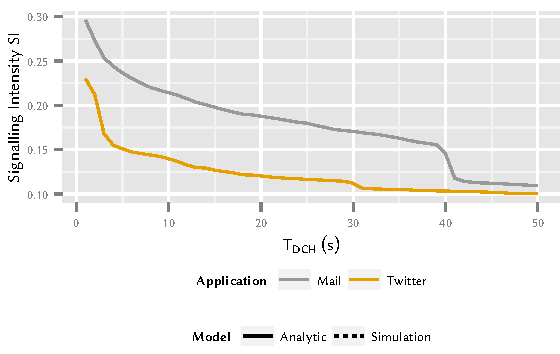
\includegraphics{network/performance_model/numerical_examples/figures/3state_tdch_si_analytic_simulative}
	\caption{Signalling intensity}\label{fig:network:performance_model:numerical_examples:validations:analytic_vs_simulation:signalling_intensity}
	\end{subfigure}

	\begin{subfigure}[b]{\textwidth}
	\centering
	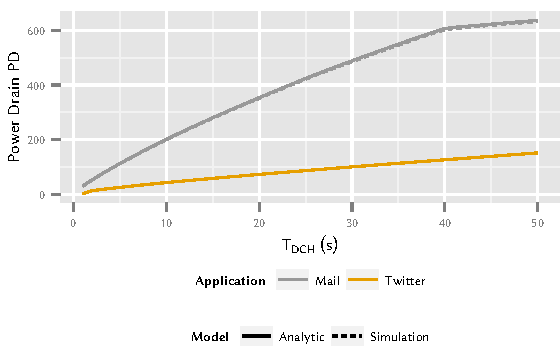
\includegraphics{network/performance_model/numerical_examples/figures/3state_tdch_pd_analytic_simulative}
	\caption{Power drain}\label{fig:network:performance_model:numerical_examples:validations:analytic_vs_simulation:power_drain}
	\end{subfigure}

	\caption{Comparison of the performance model with a \headershortacr{3G} simulation for the Three State Scenario. Lines overlap due to good fit.}\label{fig:network:performance_model:numerical_examples:validations:analytic_vs_simulation}
\end{figure}

\subsubsection*{Impact of Traffic Patterns on Signalling Intensity}\label{sec:network:performance_model:signalling_intensity}
First, we focus on the signalling intensity \(\gls{SI}\) of traffic patterns and check the impact of the average inter-packet time \(E[\PacketIAT]\) and the timer configuration. The signalling intensity \(\gls{SI}\), i.e., the average number of state transitions required for the transmission of a single packet, is an abstract measure for the signalling load produced by a specific traffic pattern.

\paragraph*{Impact of the Average Inter-Packet Time \(E[\PacketIAT]\)}\label{sec:network:performance_model:signalling_intensity:ea}
Some applications, for example those downloading or streaming of videos, send and receive large amounts of data within short time frames.
In contrast, other applications, e.g. social network clients send and receive small amounts of data every few minutes over the time span of some hours or days.

In this section we study the impact of average inter-packet times \(E[\PacketIAT]\) and the burstiness of the traffic pattern, i.e., the coefficient of variation 
\[c_{\PacketIAT} = \frac{\sqrt{\mathrm{Var}[\PacketIAT]}}{\mathrm{E}[\PacketIAT]}\]
 on the signalling load.
For that purpose, we use the simple Two State Model, set the timer \(\gls{TDCH}=\SI{10}{\second}\), consider only the first and the second moment of the inter-packet time \(\PacketIAT\), and assume that \(\PacketIAT\) follows a log-normal distribution, where both moments can be varied independently.

\begin{figure}
	\centering
	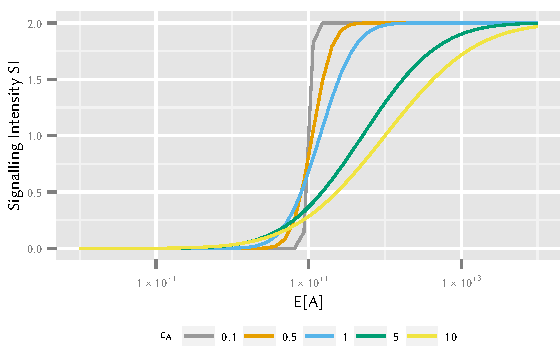
\includegraphics{network/performance_model/numerical_examples/figures/2state_ea_si}
	\caption{Signalling intensity \gls{SI} for different traffic patterns considering the Two State Model with \(\headershortacr{TDCH}=\SI{10}{\second}\) for different traffic patterns.}
	\label{fig:network:performance_model:numerical_examples:validations:analytic_vs_simulation:2state_ea_si}
\end{figure}

In \reffig{fig:network:performance_model:numerical_examples:validations:analytic_vs_simulation:2state_ea_si}, we vary the average inter-packet time \(E[\PacketIAT]\) in six orders of magnitude and investigate the resulting signalling intensity \(\gls{SI}\) for different coefficients of variation \(c_{\PacketIAT}\).
We observe that \(c_{\PacketIAT}\) has no impact on \(\gls{SI}\) for very small inter-packet times \(E[\PacketIAT]<\SI{1e-1}{\second}\).
Here, the \gls{UE} stays in state \gls{RRC_DCH} for the complete time since no inter-packet times \(\PacketIAT>\gls{TDCH}\) occur.
In addition, the impact of \(c_{\PacketIAT}\) is small for very large values of \(E[\PacketIAT]>\SI{1e3}{\second}\).
In this case, the \gls{UE} switches to state \gls{RRC_DCH} and back to state \gls{RRC_idle} for the transmission of every packet. Therefore, the signalling intensity \(\gls{SI}\) approaches the value 2.
For values in between these two extremes, the coefficient of variation \(c_{\PacketIAT}\) has a considerable impact on the signalling intensity \(\gls{SI}\).
More periodic traffic, i.e. smaller values of \(c_{\PacketIAT}\), results in an increase of \(\gls{SI}\) from 0 to 2 very sharp at the value \(E[\PacketIAT]=\gls{TDCH}\), while this increase is more smooth for larger values of \(c_{\PacketIAT}\).
This is due to the fact that for nearly periodic traffic it is crucial whether the timer value \(\gls{TDCH}\) is smaller or larger than \(E[\PacketIAT]\). 
For larger values of \(c_{\PacketIAT}\) this dependency is weaker.

\paragraph*{Impact of the Coefficient of Variation of the Inter-Packet Time \(c_\PacketIAT\)}

Next, we focus on the impact of the timer value \(\gls{TDCH}\) with respect to the burstiness of the traffic.
We use the same setting as before, but fix the average inter-packet time \(E[\PacketIAT]=\SI{4}{\second}\).
While there are differences in \(E[\PacketIAT]\) among users in real world settings, measurement studies have revealed that across all users \(\SI{95}{\percent}\) of the packets are received or transmitted within \(\SI{4.5}{\second}\) of the previous packet \cite{Falaki2010a}.
Therefore, the order of magnitude of \(E[\PacketIAT]=\SI{4}{\second}\) is of practical relevance. 

\begin{figure}
	\centering
	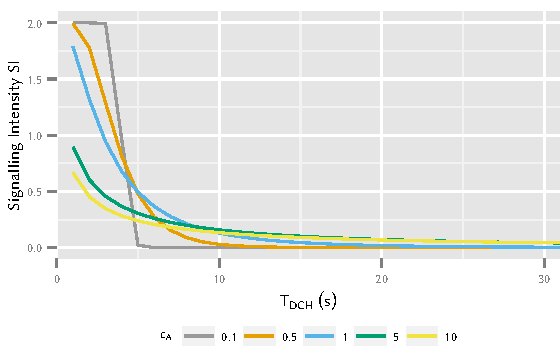
\includegraphics{network/performance_model/numerical_examples/figures/2state_tdch_si}
	\caption{Signalling intensity \(\headershortacr{SI}\) for the Two State Model w.r.t. different timeout values \(\headershortacr{TDCH}\) and coefficient of variations \(c_{\PacketIAT}\).}
	\label{fig:network:performance_model:numerical_examples:validations:analytic_vs_simulation:2state_tdch_si}
\end{figure}


The signalling intensity \(\gls{SI}\) is shown in \reffig{fig:network:performance_model:numerical_examples:validations:analytic_vs_simulation:2state_tdch_si} with respect to the timer value \(\gls{TDCH}\) and the burstiness \(c_{\PacketIAT}\) of the traffic pattern.
Obviously, larger timers lead to less frequent state transitions and therefore to less signalling load.
We observe in addition that the impact of the timer is crucial for nearly periodic traffic.
If the average inter-packet time for nearly periodic traffic is larger than the timer, then every packet transmission involves a state transitions from \gls{RRC_idle} to \gls{RRC_DCH} and a transition back.
In contrast, no transitions are required if the average inter-packet time is shorter than the timer.
With increasing values of \(c_{\PacketIAT}\) the impact of the timer is reduced.
This means that for bursty traffic patterns the timer value is of less importance with respect to the generated signalling load.

\subsubsection*{Impact of Traffic Patterns on Power Drain of the \headershortacr{UE}}\label{sec:network:performance_model:power_drain}
In this section we study the impact of the traffic patterns on the power drain \(\gls{PD}\) of the \gls{UE}.
This metric quantifies how resource-efficient specific traffic patterns and timer configurations are for the battery of the \gls{UE}.

\begin{figure}
	\centering
	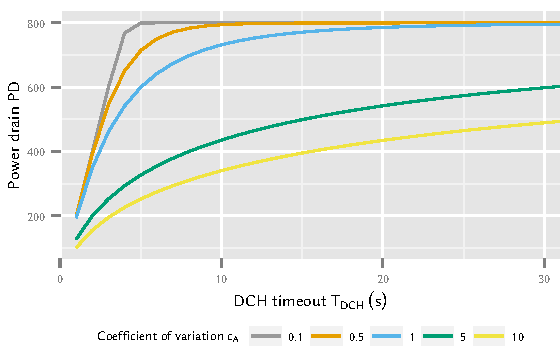
\includegraphics{network/performance_model/numerical_examples/figures/2state_tdch_pd}
	\caption{Power drain \(\headershortacr{PD}\) for the Two State Model w.r.t. different timeout values \(\headershortacr{TDCH}\) and coefficient of variations \(c_{\PacketIAT}\).}
	\label{fig:network:performance_model:numerical_examples:validations:analytic_vs_simulation:2state_tdch_pd}
\end{figure}

For the power drain in the different \gls{RRC} states, we use the same radio network power drain  used in \refsec{sec:network:network_traces:calculating_metrics}.
We investigate the impact of the average inter-packet time, the impact of the timer configuration and validate our model with simulations. 
In \refsec{sec:network:performance_model:signalling_intensity:ea} we have seen that no state transitions occur for very small and very large average inter-packet times \(E[\PacketIAT]\).
This was due to the fact that for very small values the \gls{UE} is continuously in state \gls{RRC_idle} and for large values it switches to state \gls{RRC_DCH} for every packet.
Thus, traffic patterns with very small and very large inter-packet times \(E[\PacketIAT]\) have also no impact on the power drain of the \gls{UE} regardless of the burstyness represented by the coefficient of variation \(c_{\PacketIAT}\).

To study the impact of the timer configuration \(\gls{TDCH}\), we use the same setting as for the signalling load: log-normal distribution of inter-packet time \(\PacketIAT\), \(E[\PacketIAT] = \SI{4}{\second}\) in the Two State Model.
The numerical values shown in \reffig{fig:network:performance_model:numerical_examples:validations:analytic_vs_simulation:2state_tdch_pd} indicate that longer timeouts lead to a higher power drain \(\gls{PD}\).
This is reasonable since the UE stays longer in the power intensive \gls{RRC_DCH} state in these cases.
However, we observe that the burstiness of the traffic pattern has also a considerable impact on the power drain \gls{PD}. 
For example, for \(\gls{TDCH} = \SI{15}{\second}\), the power drain is only \(\SI{400}{\milli\watt}\) for very bursty traffic with \(c_{\PacketIAT} = 10\), while it is almost \(\SI{400}{\milli\watt}\) for less bursty traffic with a \(c_{\PacketIAT} = 1\). 
The reason is that bursty traffic patterns send a lot of traffic during short periods when the UE is in state \gls{RRC_DCH} anyway. During the following off-periods that \gls{UE} can save power in \gls{RRC_idle} state.
Hence, we conclude that longer timeouts and smaller coefficients of variation \(c_{\PacketIAT} = 1\), i.e. more periodic and less bursty traffic, result in a higher power drain of the \gls{UE}.

\subsubsection*{Tradeoff: Energy Consumption vs. Signalling Load}\label{sec:network:performance_model:trade_off}
In \reffig{fig:network:performance_model:numerical_examples:validations:analytic_vs_simulation:2state_pd_vs_si_vs_tdch}, we show the effect of network parameter optimisation using the timer \gls{TDCH} on traffic patterns with varying coefficient of variation.

\begin{figure}
	\centering
	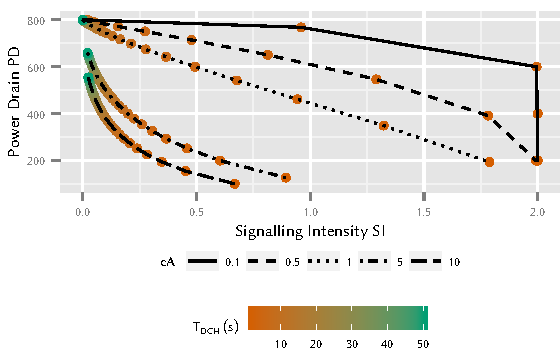
\includegraphics{network/performance_model/numerical_examples/figures/2state_pd_vs_si_vs_tdch}
	\caption{Trade-off between \(\headershortacr{PD}\) and \headershortacr{SI} for the Two State Model.}
	\label{fig:network:performance_model:numerical_examples:validations:analytic_vs_simulation:2state_pd_vs_si_vs_tdch}
\end{figure}

We see that optimisations may decrease signalling by large amounts while only having very little impact on power drain for one specific kind of traffic.
The same timer setting could increase the power drain for another kind of traffic while only offering little benefit with regard to the generated signalling intensity.
